\section{Progrès réalisé}

\subsection{IA - Intelligence artificielle}
\setlength{\parindent}{5ex}
Lorem ipsum dolor sit amet, consectetur adipiscing elit. Integer fermentum eros sed neque aliquet fermentum. Ut aliquam placerat velit. Vestibulum ante ipsum primis in faucibus orci luctus et ultrices posuere cubilia curae; Etiam interdum in erat vitae convallis. Nullam sed mauris in ex porta auctor. Aenean in lobortis mi. Nam molestie felis sit amet maximus congue. Aenean rhoncus, libero nec suscipit aliquam, risus velit ultricies est, at vestibulum ipsum elit sed risus. In malesuada efficitur ipsum vel vestibulum. Integer sed mi nec augue laoreet efficitur vel et risus. Quisque pharetra nunc elit.

\subsection{Audio et Effets Sonores}
\setlength{\parindent}{5ex}
Pour l’audio, la cinématique principale et le menu d’accueil du jeu comptent déjà avec ses propres musiques, libres de droits et utilisables pour usage commercial, qui représentent bien l’aspect mystérieux et effrayant de notre jeu d’horreur.

Les effets sonores du menu d’accueil ont déjà été mis en place et les effets extradiégétiques trouvables dans le jeu ont déjà été sélectionnés (ramassage d’objets, interaction quelconque).

Nous continuons d’effectuer des recherches concernant les effets sonores liés aux différents matériaux du jeu lorsque les joueurs y marchent dessus. Cependant, les effets sonores gratuits seront très accessibles grâce aux bibliothèques d’effets sonores gratuits \emph{Zapsplat} ou \emph{Freesound} auxquelles on a déjà jeté un coup d’œil. 


\subsection{Gameplay}
\setlength{\parindent}{5ex}
Concernant les contrôles en jeu du personnage, le début a demandé beaucoup de recherches, n’étant pas familier avec Unity3D. Nous avons d’abord opté pour une gestion des contrôles en utilisant le système des « presskey » et nous avons implanté les déplacements, le saut, la course et s'accroupir, puis d’autres recherches ont été nécessaire pour la gestion de la caméra à la première personne. La caméra a été placée dans la tête du modèle, est gérée avec la souris et est limitée, en partant d’une vue au centre, à quatre-vingt-dix degrés vers le haut et le bas, quand la souris est bougée horizontalement, le corps du modèle tourne.
\newline
\vfill
\noindent\makebox[\linewidth]{\rule{.8\paperwidth}{.6pt}}\\[0.2cm]
EPITA Toulouse - Projet S2 - 2022 \hfill Nyctalopia - gameHUB
\noindent\makebox[\linewidth]{\rule{.8\paperwidth}{.6pt}}

\newpage

Il a donc fallu par la suite implémenter le fait que en maintenant la touche « avancer » ou « reculer » et tourner la caméra horizontalement, le personnage continue de marcher vers la direction de la tête. Ensuite nous nous sommes rendu compte qu’il fallait garder le curseur au milieu de l’écran ce qui a été fait assez facilement avec quelques recherches.

Par la suite, nous avions en tête d’implémenter un système permettant de pouvoir changé les touches liées aux actions. Après des recherches sur le sujet nous nous sommes rendu compte que le système précédemment expliqué pour gérer les contrôles du personnage ne permettait pas de faire cela. Nous avons donc opté pour l’utilisation du ``New Input System''  de Unity3D.

Il nous a donc fallut réimplémenter les contrôles avec ce nouvel outil qui fut assez compliqué à prendre en main, comme les ressources disponibles sur internet sont moins riches que pour les précédant système de gestion d’entrée. Cependant, une fois compris ce système est bien plus facile et efficace, de plus celui-ci nous permet laisser à l’utilisateur le choix de ses touches et de pouvoir facilement changer les touches utilisées et détectées selon le statut du jeu : en jeu/dans les menus.

Ensuite nous avons choisi de supprimer l’action de course et de saut pour mieux coller à l’ambiance du jeu, le rendant plus oppressant du fait de nos mouvements limités. La gestion de l’action « s’accroupir » a aussi été revu car peu compréhensible dans le code et ne fonctionnant pas bien.

Après quelques tests, nous nous sommes aussi rendu compte que le curseur restait bloqué. Nous avons donc rajouté sur la touche « escape », sur les contrôles en jeu, le fait que le curseur redevenait libre et les contrôles passent du mode « en jeu » au mode « menu ».
Concernant la partie pour laisser le joueur choisir ses touches, nous sommes partis d’un code type de la documentation Unity3D expliqué à l’aide d’une vidéo.

Nous nous sommes ensuite rendu compte que pour l’adapter à notre menu on devait mettre plusieurs paramètres dans une fonction appelé par un bouton. Nous avons donc codé un script pour le bouton à la place d’utilisé l’inspecteur de Unity3D.

Nous avons pu coder ses scripts en nous aidant de la documentation Unity, de vidéos explicatives et de forum.

Voici le code des contrôle en jeu appelés à l'aide du ``New Input System'' :
\newline

\begin{lstlisting}[language={[Sharp]C}, caption={Fonctions C\# Awake / Update}, label={Script}]
void Awake()
{
	playerCamera = GetComponentInChildren<Camera>();
}

private void Update()
{
	if (controller.isGrounded)
	{
		movementSpeed = isCrouching ? crouchSpeed : walkSpeed;
		finalMovement = transform.TransformDirection(inputMovement) * movementSpeed * Time.deltaTime;
	}

	finalMovement.y -= gravity * Time.deltaTime;
    controller.Move(finalMovement);
}
\end{lstlisting}
La fonction ``Awake'' permet de récupérer la caméra du joueur lorsque l'on initialise le script.
La fonction ``Update'' est appelée à chaque image et va être responsable du mouvement du joueur.
``movementSpeed'' donne la vitesse du joueur et change si celui-ci est accroupi ou non.
``finalMovement'' donne le mouvement final seulement au sol en fonction de la fonction ``Move'' qui sera traitée ci-dessous.
Enfin, dans tout les cas, on va appliquer un mouvement négatif en y qui simule la gravité.
``controller.Move()'' applique les mouvement précédemment définit au joueur.
\newline

\begin{lstlisting}[language={[Sharp]C}, caption={Fonction C\# Move}, label={Script}]
public void Move(InputAction.CallbackContext ctx)
{
    var inputValue = ctx.ReadValue<Vector2>();
    inputMovement = new Vector3(inputValue.x, 0f, inputValue.y);
}
\end{lstlisting}
La fonction ``Move'', va lire en entrée les touches responsable du déplacement, de base ``ZQSD'', et va les assigner à la variable ``inputvalue'' qui est utilisée dans la fonction ``Update'' vu précédemment.
\newline

\begin{lstlisting}[language={[Sharp]C}, caption={Fonction C\# Crouch}, label={Script}]
public void Crouch(InputAction.CallbackContext ctx)
{
    if (!ctx.performed) {return; }
	if (isCrouching)
	{
		if (isCrouching && Physics.Raycast(playerCamera.transform.position, Vector3.up, standingHeight - crouchingHeight))
		// Permet de savoir si un objet se trouve au dessus du joueur quand celui-ci est accroupi
		{
			//Debug.Log("Error");
			return;
		}
		else
		{
			//Debug.Log("Standing");
			isCrouching = false;
			controller.height = standingHeight;
		}
	}
	else
	{
		//Debug.Log("Crouching");
		isCrouching = true;
		controller.height = crouchingHeight;
	}
}
\end{lstlisting}
La fonction ``Crouch'' lit l'entrée de la touche responsable de l'action s'accroupir, par défaut ``Shift''. Elle va baisser le joueur et son masque de collision jusqu'à une valeur donnée correspondant à l'animation du modèle et va changer la vitesse. Lorsque le joueur réappuie sur la touche la fonction va vérifier si un objet se trouve au dessus de lui, si il ni en à pas la hauteur est remise à la normale.
\newline

\begin{lstlisting}[language={[Sharp]C}, caption={Fonction C\# Escape}, label={Script}]
public void Escape(InputAction.CallbackContext ctx)
		{
			if (!ctx.performed) {return; }
			Cursor.lockState = CursorLockMode.None;
			PlayerInput.actions.FindActionMap("Gameplay").Disable();
			PlayerInput.actions.FindActionMap("Menu").Enable();
			CameraInput.actions.FindActionMap("Gameplay").Disable();
			CameraInput.actions.FindActionMap("Menu").Enable();
		}
\end{lstlisting}
La fonction ``Escape'' permet de libérer le curseur et change les contrôles de ``en jeu'' à ``menu''.
Voici le script permettant de dirigé la caméra :
\newline

\begin{lstlisting}[language={[Sharp]C}, caption={Fonction C\# Caméra}, label={Script}]
void Start()
{
    Cursor.lockState = CursorLockMode.Locked; //Garde le curseur au centre de l'écran
}
    
void Update()
{
        
    float mouseX = looking.x * mouseSensitivity * Time.deltaTime;
    float mouseY = looking.y * mouseSensitivity * Time.deltaTime;

    xRotation -= mouseY;
    xRotation = Math.Clamp(xRotation, -90f, 90f); //Limite la rotation de la caméra
        
    transform.localRotation = Quaternion.Euler(xRotation, 0, 0); //Tourne la caméra
    playerBody.Rotate(Vector3.up * mouseX); //Tourne le corps
}

public void Look(InputAction.CallbackContext ctx)
{
	looking = ctx.ReadValue<Vector2>();
}
\end{lstlisting}
\vfill
\noindent\makebox[\linewidth]{\rule{.8\paperwidth}{.6pt}}\\[0.2cm]
EPITA Toulouse - Projet S2 - 2022 \hfill Nyctalopia - gameHUB
\noindent\makebox[\linewidth]{\rule{.8\paperwidth}{.6pt}}
\newpage
La fonction ``Start'' permet de bloquer le curseur au milieu de l'écran avant d'enregistrer les entrée souris.
La fonction ``Update'' va récupérer les entrée lu par la fonction ``Look'' et appliquer ces changement à la caméra qui est bloquée comme évoqué précédemment.
``playerBody.Rotate'' permet de pouvoir maintenir la touche avancé et de suivre la direction pointée par la caméra.

\subsection{Communication}
\setlength{\parindent}{5ex}
Pour le logo du studio, nous avons opté pour un logo s’inspirant du logo de la plateforme GitHub, en le stylisant pour le faire correspondre au thème de notre jeu. En effet on peut y voir la silhouette d’une chouette devant une pleine lune. Nous avons fait des tests avec plusieurs silhouettes d’animaux notamment des corbeaux et des chouettes, qui représente le thème de la nuit.

\newline
Finalement nous avons opté pour la chouette qui rendais le mieux car occupe un assez grand espace dans le cercle, est assez ronde et est entièrement visible.
Concernant le logo du jeu, nous avons opté pour un style simple en stylisant la lettre « N », première lettre du nom du jeu.

\newline
\begin{figure}[H]
\centering
\begin{minipage}{.5\textwidth}
  \centering
  \centerline{
\includegraphics[width=0.5\linewidth]{img/logos/logojeu.png}}
  \captionof{figure}{\emph{Logo Nyctalopia}}
  \label{fig:logonyctalopia}
\end{minipage}%
\end{figure}

\vfill
\noindent\makebox[\linewidth]{\rule{.8\paperwidth}{.6pt}}\\[0.2cm]
EPITA Toulouse - Projet S2 - 2022 \hfill Nyctalopia - gameHUB
\noindent\makebox[\linewidth]{\rule{.8\paperwidth}{.6pt}}

\subsection{Graphismes, Modèles et Terrain}
\setlength{\parindent}{5ex}
Nous avons décidé de générer un terrain de manière procédurale à l'aide d'une bibliothèque de génération de terrain et ensuite le modifier selon notre convenance pour obtenir ce côté réaliste d'une forêt en montagne.

Une grande variété de modèles 3D d’arbres, arbustes et herbe ont déjà été sélectionnés et utilisés dans le jeu pour couvrir ce terrain et créer une forêt riche et variée. La plupart de ces modèles de végétation proviennent de la bibliothèque de modèles 3D \emph{Quixel’s Megascans} et du site officiel de modèles Unity \emph{Unity Asset Store}. Plusieurs modifications et conversions ont été nécessaires pour les rendre compatibles avec notre projet qui est basé sur le système de rendu HDRP (\emph{High-Definition Render Pipeline}) qui offre des résultats graphiques plus attractifs.
\newline

L'histoire du jeu se basera sous forme de chapitres, pour l'instant, nous n'avons réalisé qu'une cinématique : Chapitre 0 : Dark Night.
\newline

\begin{figure}[H]
\centering
\begin{minipage}{.5\textwidth}
  \centering
  \centerline{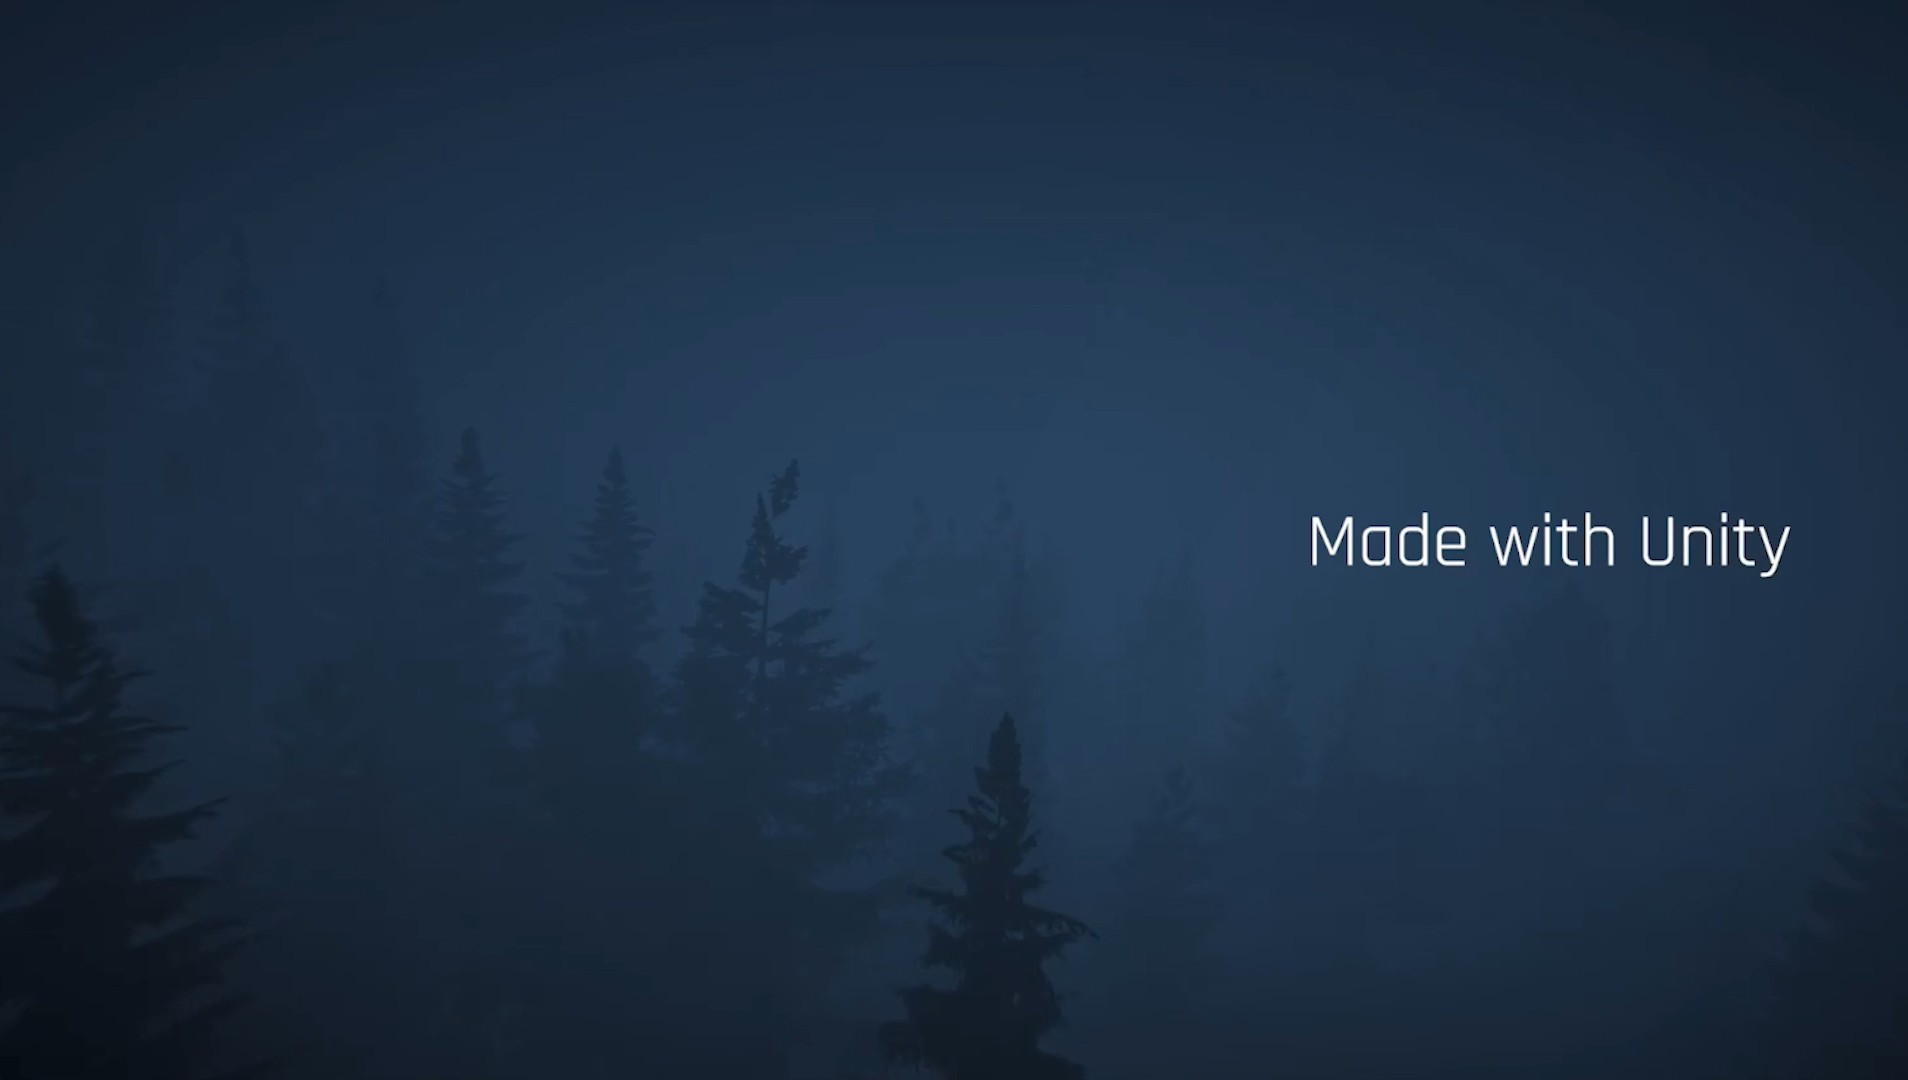
\includegraphics[width=1\linewidth]{img/cine.png}}
  \captionof{figure}{\emph{Chapitre 0 : Dark Night}}
  \label{fig:cinematique}
\end{minipage}%
\end{figure}

Nous aurons ensuite une partie qui se déroulera dans la forêt (Chapitres 1 et 2), puis un troisième dans des souterrains.
\newline

\begin{figure}[H]
\centering
\begin{minipage}{.5\textwidth}
  \centering
  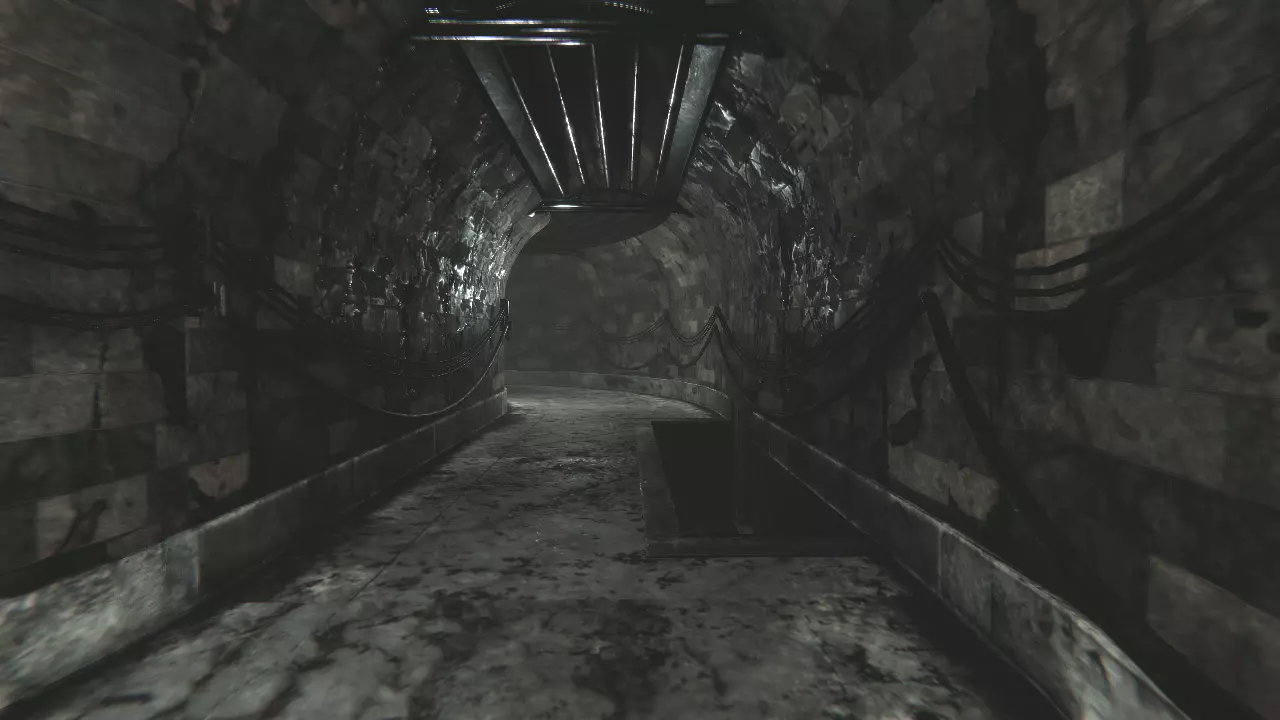
\includegraphics[width=.6\linewidth]{img/assets/egouts1.png}
  \captionof{figure}{\emph{Représentation du Chapitre 3}}
  \label{fig:rémi}
\end{minipage}%
\begin{minipage}{.5\textwidth}
  \centering
  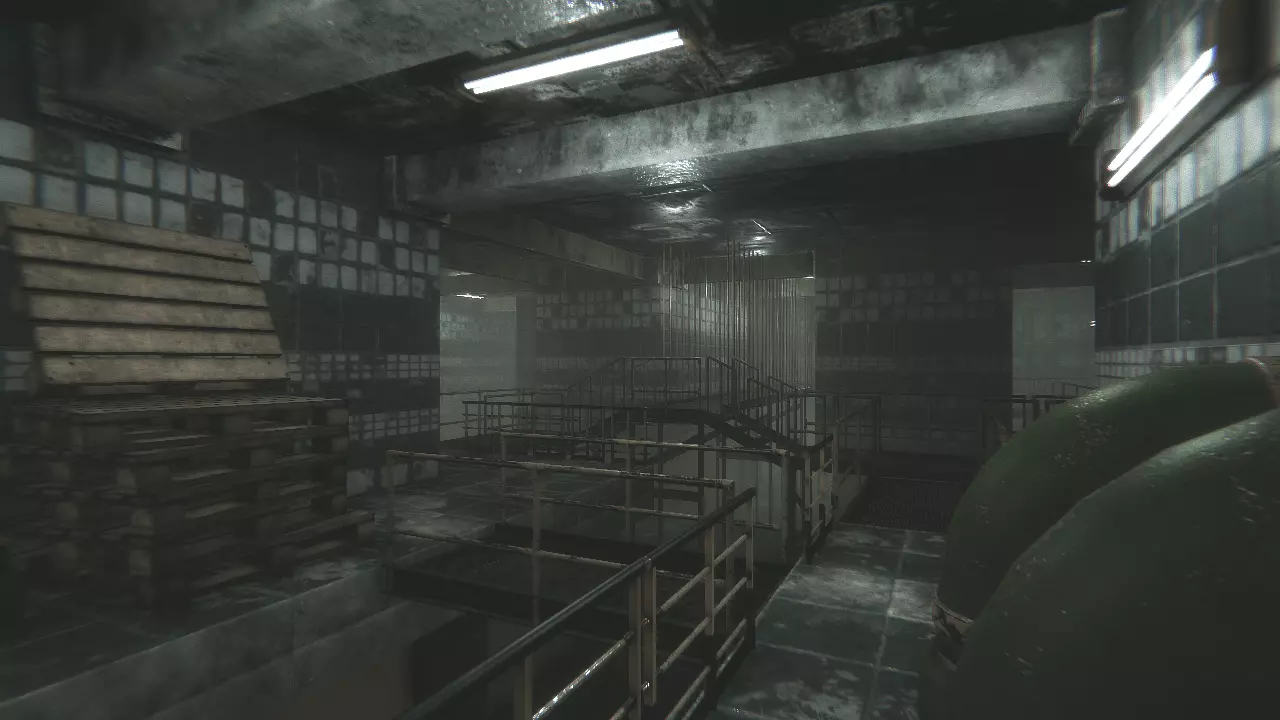
\includegraphics[width=.6\linewidth]{img/assets/egouts2.png}
  \captionof{figure}{\emph{Représentation du Chapitre 3}}
  \label{fig:sonia}
\end{minipage}
\end{figure}

\vfill
\noindent\makebox[\linewidth]{\rule{.8\paperwidth}{.6pt}}\\[0.2cm]
EPITA Toulouse - Projet S2 - 2022 \hfill Nyctalopia - gameHUB
\noindent\makebox[\linewidth]{\rule{.8\paperwidth}{.6pt}}

\newpage



Les modèles plus spécifiques telles que la route, les différentes voitures, le bâtiment et le lampadaire du lobby multijoueur proviennent des mêmes bibliothèques.
\newline

\begin{figure}[H]
\centering
\begin{minipage}{.5\textwidth}
  \centering
  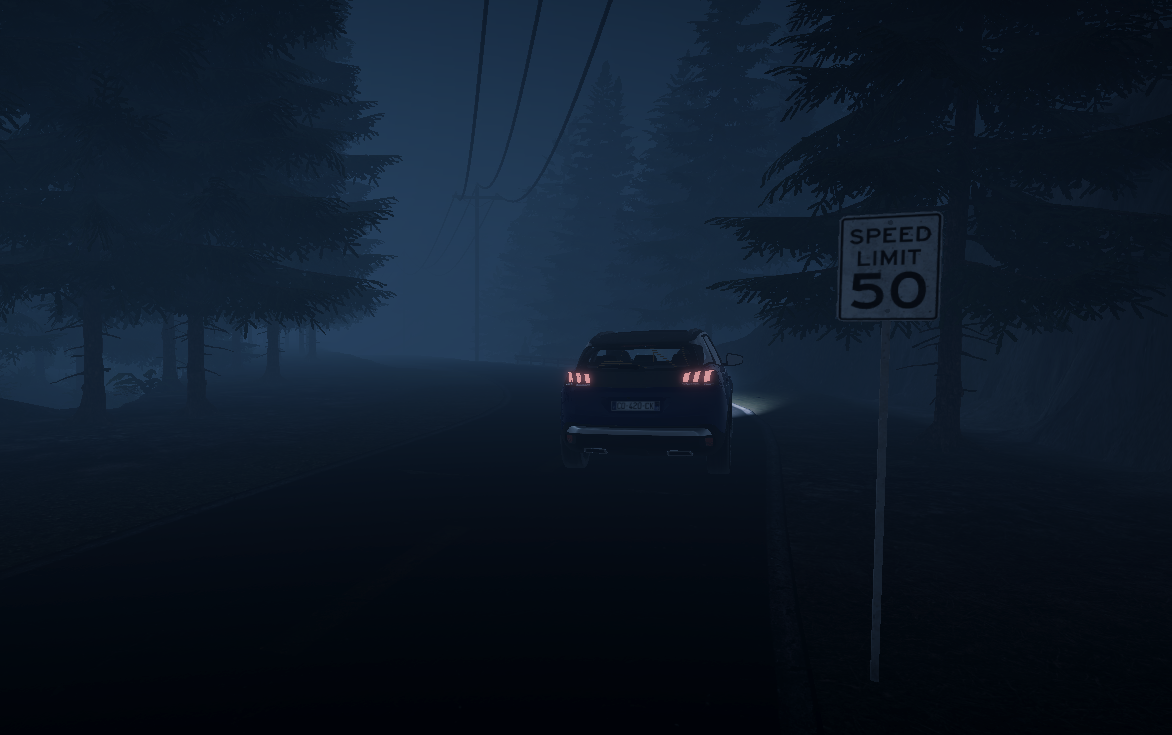
\includegraphics[width=.6\linewidth]{img/assets/car.png}
  \captionof{figure}{\emph{Voiture}}
  \label{fig:car}
\end{minipage}%
\begin{minipage}{.5\textwidth}
  \centering
  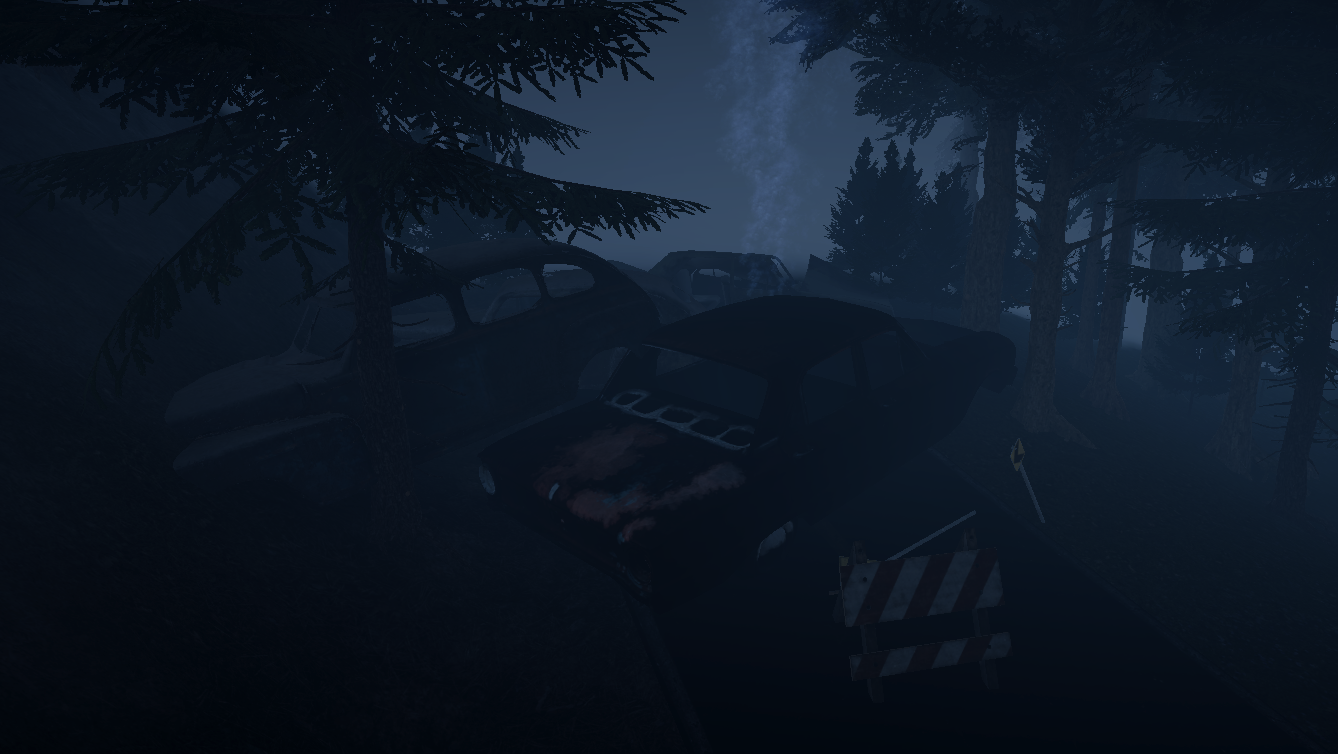
\includegraphics[width=.6\linewidth]{img/assets/crash.png}
  \captionof{figure}{\emph{Scène de l'accident}}
  \label{fig:crash}
\end{minipage}
\end{figure}

\vfill
\noindent\makebox[\linewidth]{\rule{.8\paperwidth}{.6pt}}\\[0.2cm]
EPITA Toulouse - Projet S2 - 2022 \hfill Nyctalopia - gameHUB
\noindent\makebox[\linewidth]{\rule{.8\paperwidth}{.6pt}}

\newpage

Concernant les personnages jouables, nous comptons actuellement avec deux modèles de personnages complètement animés, un homme et une femme, provenant de la bibliothèque d’Adobe \emph{Mixamo}.
\newline

\begin{figure}[H]
\centering
\begin{minipage}{.5\textwidth}
  \centering
  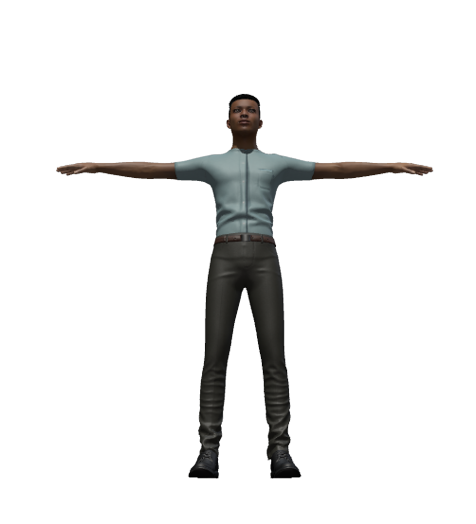
\includegraphics[width=.6\linewidth]{img/assets/remi.png}
  \captionof{figure}{\emph{Personnage masculin}}
  \label{fig:rémi}
\end{minipage}%
\begin{minipage}{.5\textwidth}
  \centering
  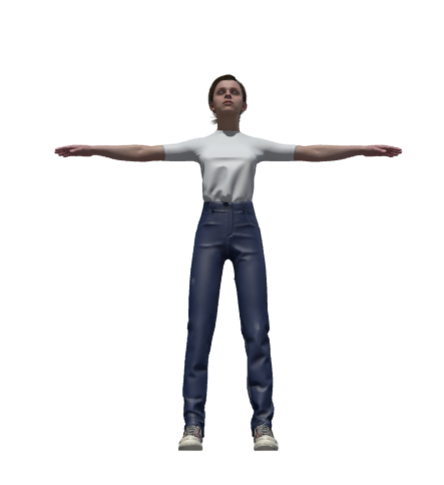
\includegraphics[width=.6\linewidth]{img/assets/sonia.png}
  \captionof{figure}{\emph{Personnage féminin}}
  \label{fig:sonia}
\end{minipage}
\end{figure}

Pour l'entité qui suivra le joueur plus tard dans le jeu, un modèle a déjà été choisi.
\newline

\begin{figure}[H]
\centering
\begin{minipage}{.5\textwidth}
  \centering
  \centerline{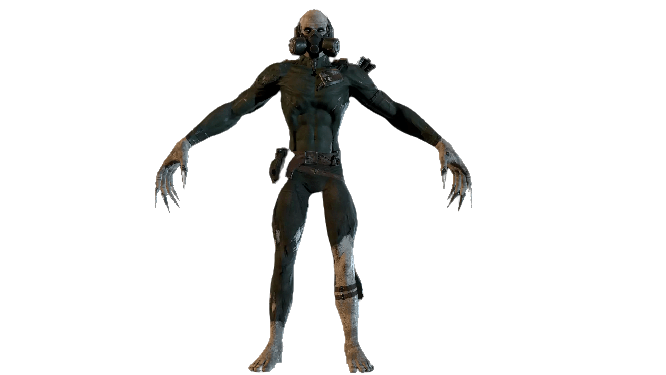
\includegraphics[width=1\linewidth]{img/assets/sterven.png}}
  \captionof{figure}{\emph{Entité}}
  \label{fig:fusebox}
\end{minipage}%
\end{figure}

\vfill
\noindent\makebox[\linewidth]{\rule{.8\paperwidth}{.6pt}}\\[0.2cm]
EPITA Toulouse - Projet S2 - 2022 \hfill Nyctalopia - gameHUB
\noindent\makebox[\linewidth]{\rule{.8\paperwidth}{.6pt}}

\newpage

\subsection{Manuels et Documentation}
\setlength{\parindent}{5ex}
Lorem ipsum dolor sit amet, consectetur adipiscing elit. Integer fermentum eros sed neque aliquet fermentum. Ut aliquam placerat velit. Vestibulum ante ipsum primis in faucibus orci luctus et ultrices posuere cubilia curae; Etiam interdum in erat vitae convallis. Nullam sed mauris in ex porta auctor. Aenean in lobortis mi. Nam molestie felis sit amet maximus congue. Aenean rhoncus, libero nec suscipit aliquam, risus velit ultricies est, at vestibulum ipsum elit sed risus. In malesuada efficitur ipsum vel vestibulum. Integer sed mi nec augue laoreet efficitur vel et risus. Quisque pharetra nunc elit.

\subsection{Multijoueur}
\setlength{\parindent}{5ex}
Pour le multijoueur nous avons décidé d'utiliser le SDK Steamworks fourni par Steam Inc. N'étant pas pas nativement compatible avec C\#, nous avons dû utiliser une bibliothèque tierce nommée {\emph{Steamworks.NET}}. Ce SDK permettra de créer des lobbys et d'intégrer une liste d'amis, qui facilitera la communication entre les deux joueurs étant donné que Steam est la plateforme de vente de jeux vidéos la plus populaire au monde avec 100+ millions de connexions mensuelles. Également, nous avons besoin :

\begin{itemize}
    \item{ D'un HLAPI, \emph{High Level Application Programming Interface} ou, interface permettant au jeu de communiquer avec les serveurs Steam. Celle-ci sera Mirror, une bibliothèque Unity open-source censé remplacer officieusement UNet.}
    \newline
    \item{ D'un LLAPI, \emph{Low Level Application Programming Interface} ou interface permettant au LLAPI de communiquer avec le HLAPI. Celui-ci sera FizzySteamworks, également Open Source et disponible sur GitHub.}
\end{itemize}

Avec tout ces outils en place, il nous a suffi de lire la documentation officielle de Steam, et de mettre en place un script consistant à créer et à joindre des lobbys grâces aux boutons présents au sein de l'interface (c.f. UI/UX).

\begin{lstlisting}[language={[Sharp]C}, caption={Fonction C\# UILinker}, label={Script}]
void Start()
{
    lobbyCreated = Callback<LobbyCreated_t>.Create(OnLobbyCreated);
    lobbyEntered = Callback<LobbyEnter_t>.Create(OnLobbyEntered);
        
    // START HOST thanks to the UIButton StartHost
    StartHost?.onClick.AddListener(() => 
    {
        CreateNewLobby(ELobbyType.k_ELobbyTypeFriendsOnly);
    });

    // START CLIENT thanks to the UIButton StartClient
    StartClient?.onClick.AddListener(() => 
    {
        JoinLobby(new CSteamID(System.Convert.ToUInt64(LobbyCSteamIDInput.text)));
    });
}
\end{lstlisting}

\vfill
\noindent\makebox[\linewidth]{\rule{.8\paperwidth}{.6pt}}\\[0.2cm]
EPITA Toulouse - Projet S2 - 2022 \hfill Nyctalopia - gameHUB
\noindent\makebox[\linewidth]{\rule{.8\paperwidth}{.6pt}}

\newpage
\begin{figure}[H]
\centering
\begin{minipage}{.5\textwidth}
  \centering
  \centerline{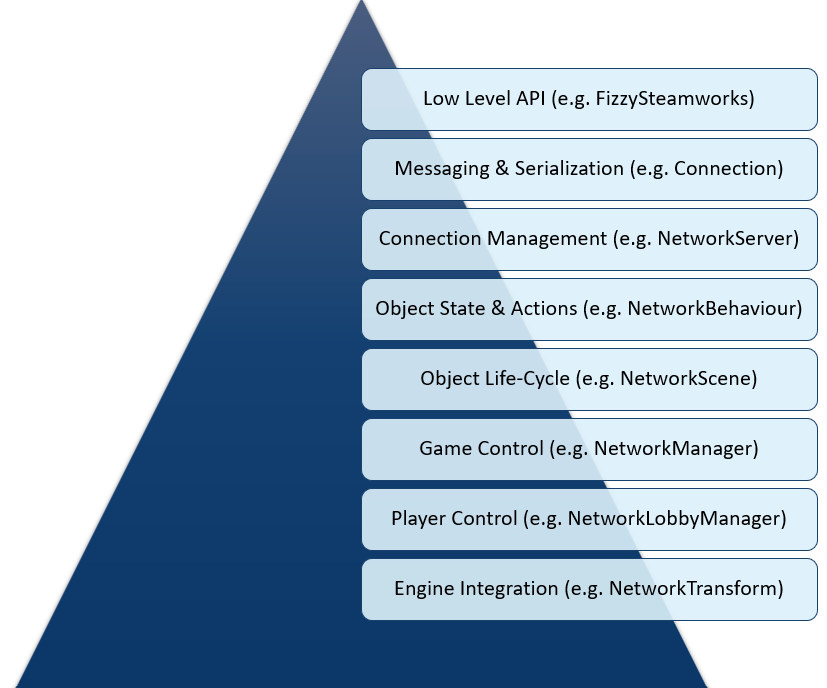
\includegraphics[width=1.5\linewidth]{img/HLAPI.png}}
  \captionof{figure}{\emph{Structure d'un HLAPI}}
  \label{fig:hlapistructure}
\end{minipage}%
\end{figure}

\vfill
\noindent\makebox[\linewidth]{\rule{.8\paperwidth}{.6pt}}\\[0.2cm]
EPITA Toulouse - Projet S2 - 2022 \hfill Nyctalopia - gameHUB
\noindent\makebox[\linewidth]{\rule{.8\paperwidth}{.6pt}}

\newpage


\subsection{UI/UX - Interface}
\setlength{\parindent}{5ex}
L'interface utilisateur possède trois parties principales, le menu principal, le menu ``Play'' et le menu ``Paramètres''. Ce dernier permet à l'utilisateur de pouvoir régler la résolution, la taille de la fenêtre (fenêtré, borderless ou plein écran), mais également le son et le choix des touches (AZERTY, QWERTY ou n'importe quelle combinaison de touches).
Le menu ``Play'' possède trois boutons, un placé à gauche, permettant au joueur 1 de créer un lobby et de le rejoindre, et à droite deux boutons permettent au joueur 2 de soit, joindre le lobby avec un \emph{CSteamID} (code de lobby délivré par Steam) ou bien en utilisant sa liste d'ami Steam.
Enfin, le menu principal possède deux grands boutons appelant le joueur à soit débuter une nouvelle campagne ou bien de continuer là où il avait sauvegardé pour la dernière fois (c.f. Sauvegardes)

\begin{figure}[H]
\centering
\begin{minipage}{.5\textwidth}
  \centering
  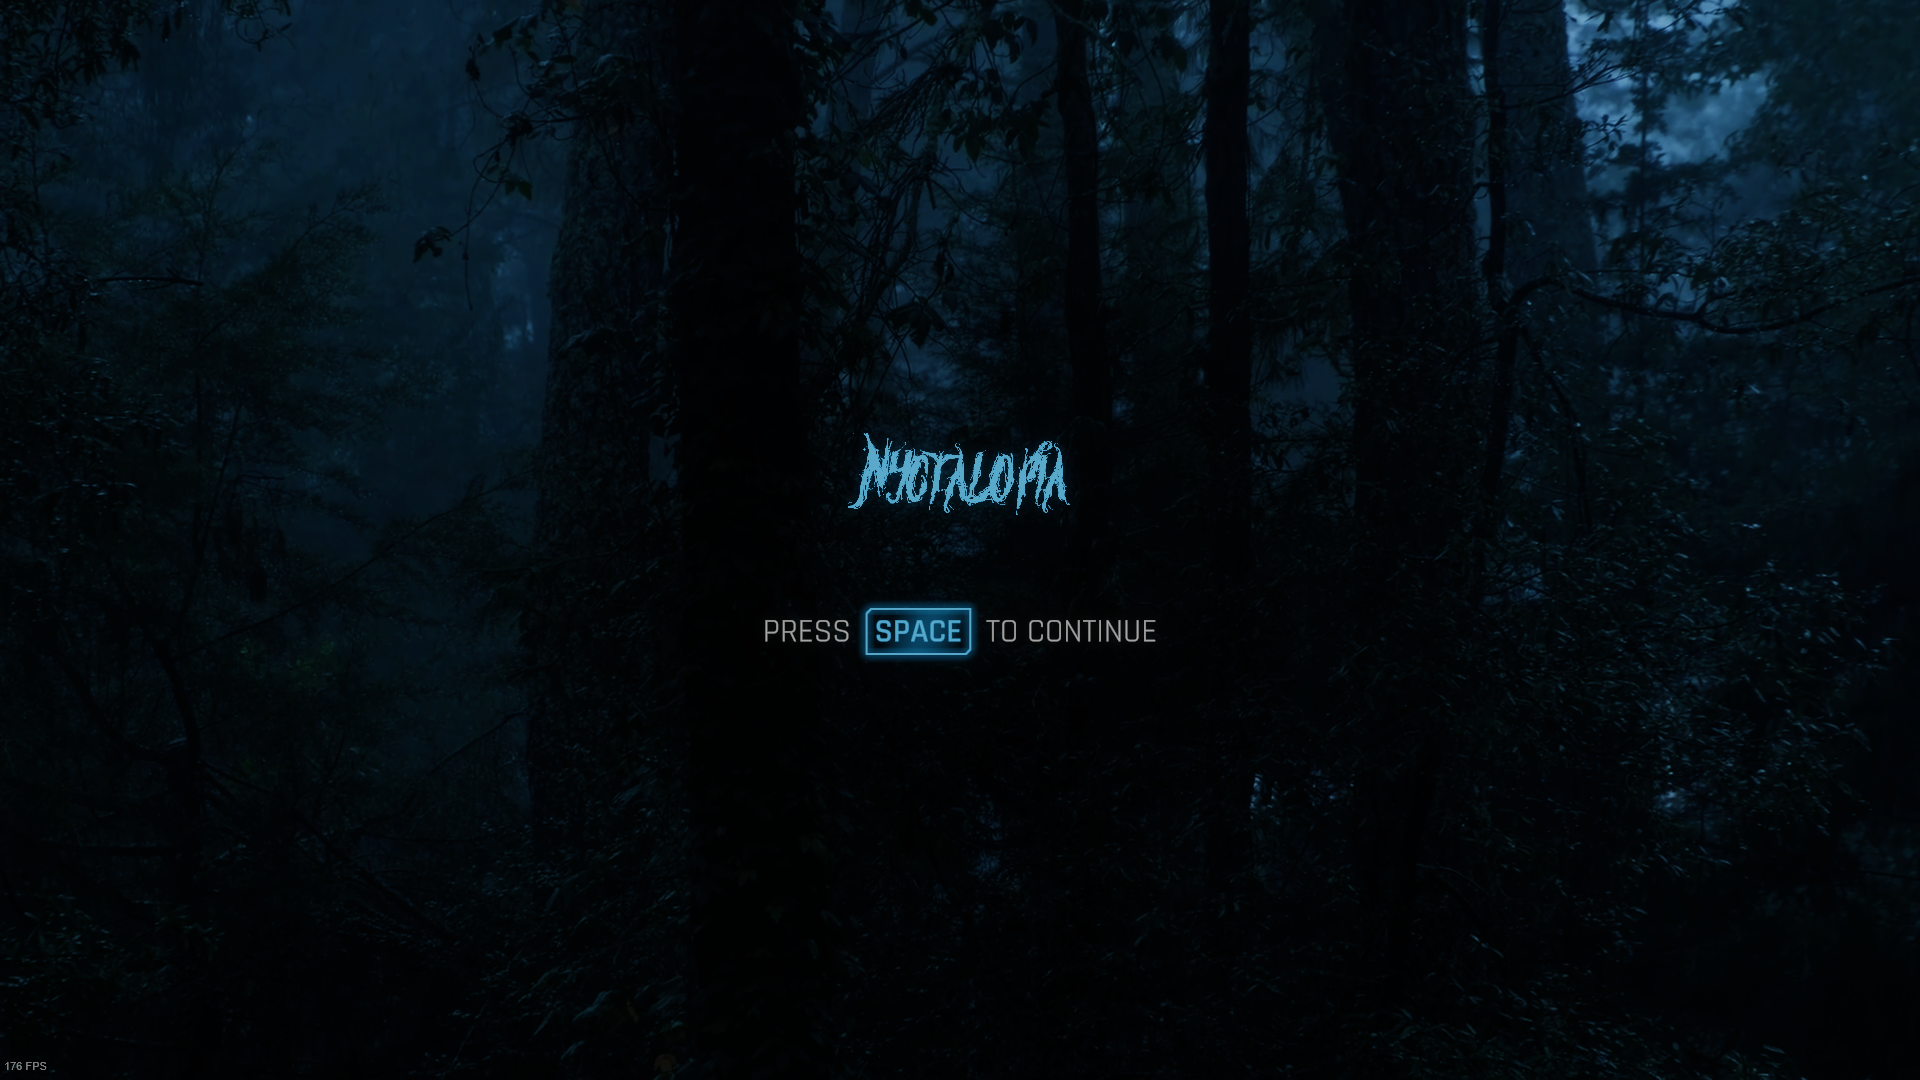
\includegraphics[width=.9\linewidth]{img/ui/UI2.png}
  \captionof{figure}{\emph{Écran d'accueil}}
  \label{fig:uihome}
\end{minipage}%
\begin{minipage}{.5\textwidth}
  \centering
  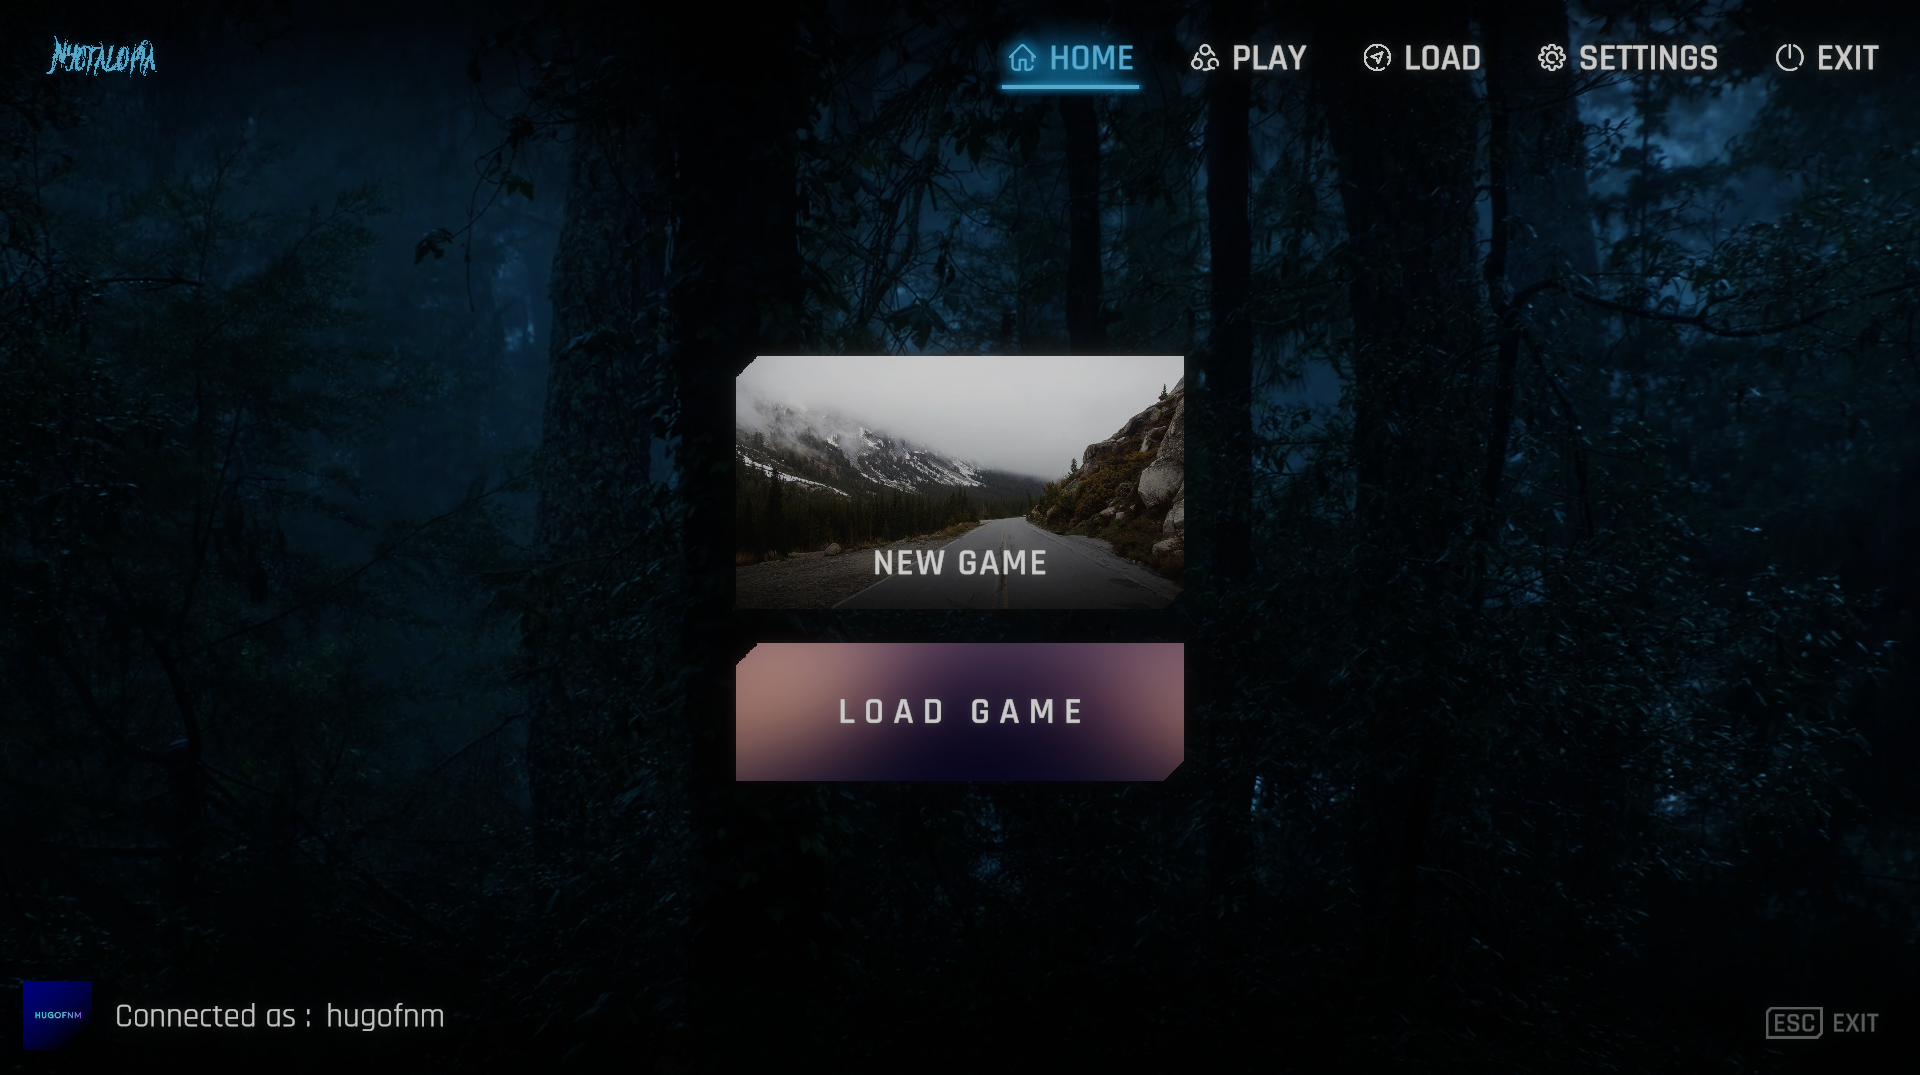
\includegraphics[width=.9\linewidth]{img/ui/UI1.png}
  \captionof{figure}{\emph{Menu principal}}
  \label{fig:uihome2}
\end{minipage}
\end{figure}

\begin{figure}[H]
\centering
\begin{minipage}{.5\textwidth}
  \centering
  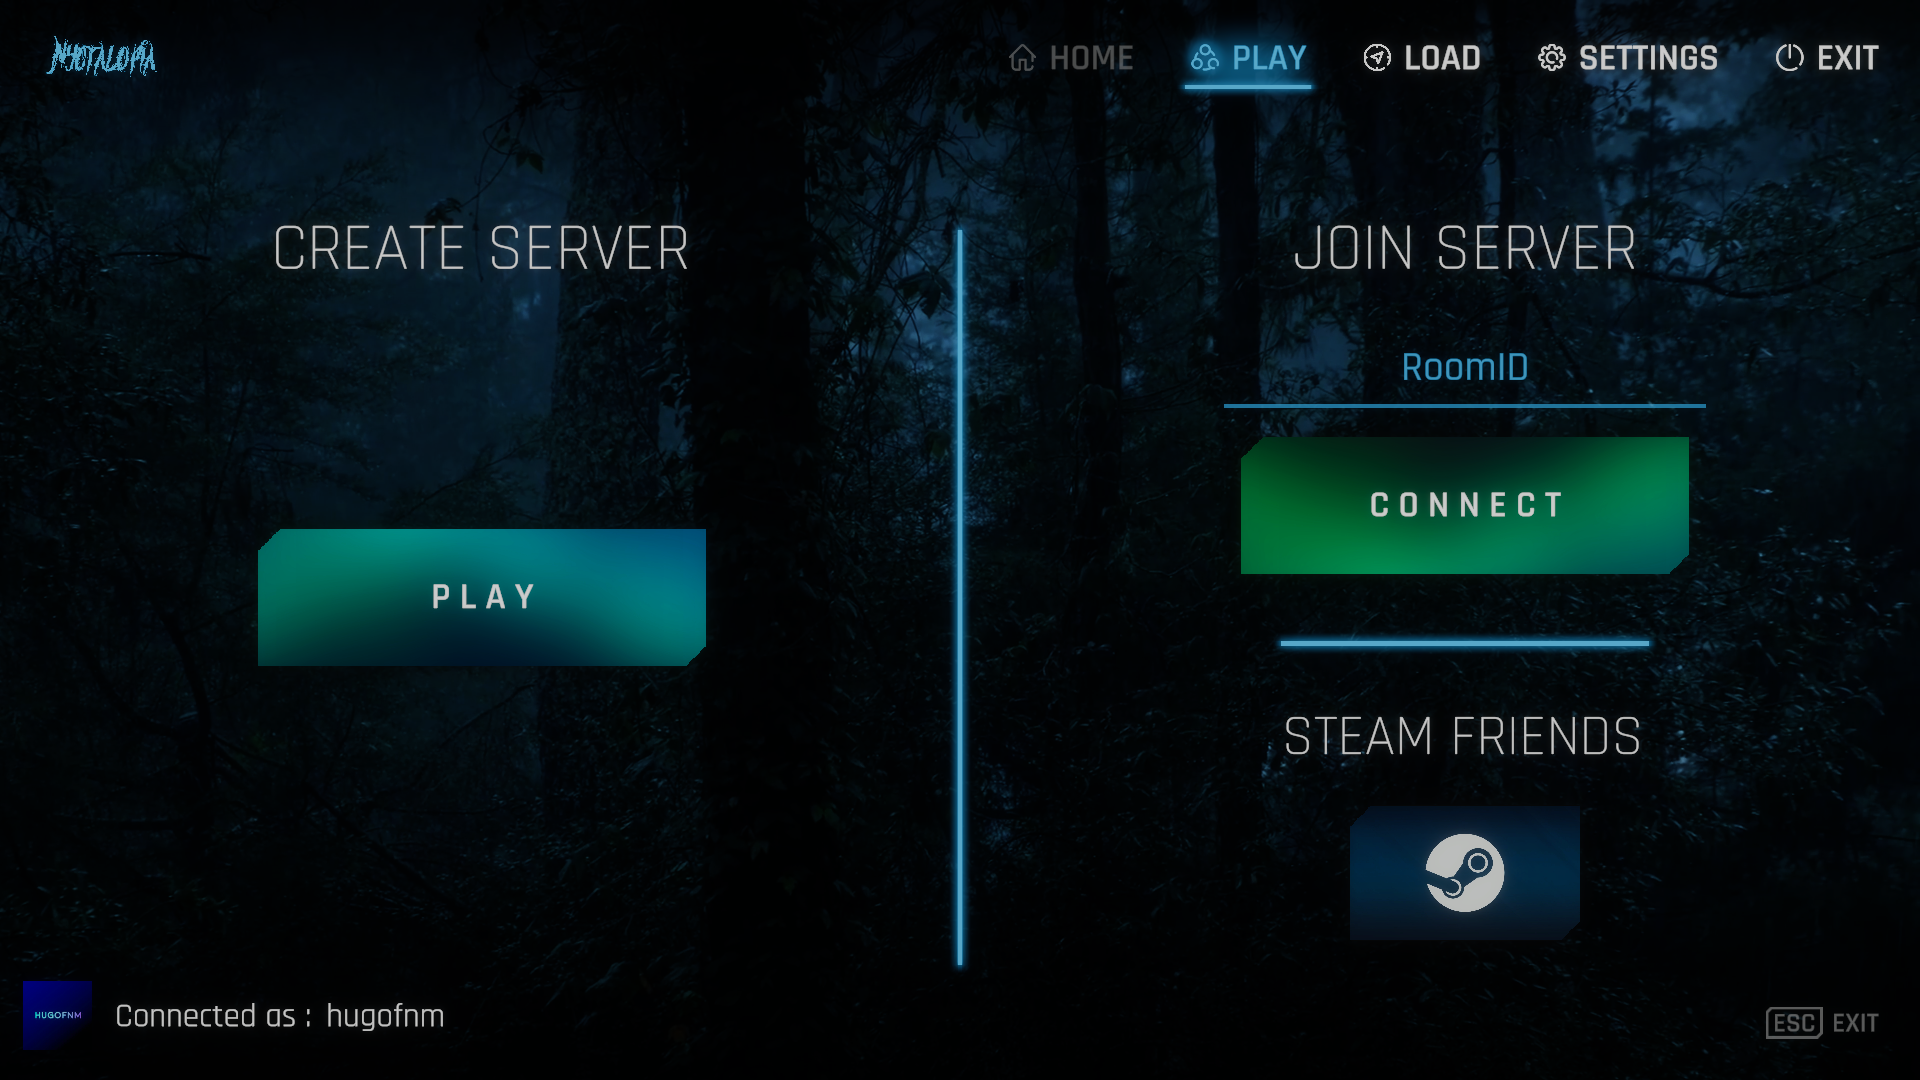
\includegraphics[width=.9\linewidth]{img/ui/UI.png}
  \captionof{figure}{\emph{Menu ``Play''}}
  \label{fig:uiplay}
\end{minipage}%
\begin{minipage}{.5\textwidth}
  \centering
  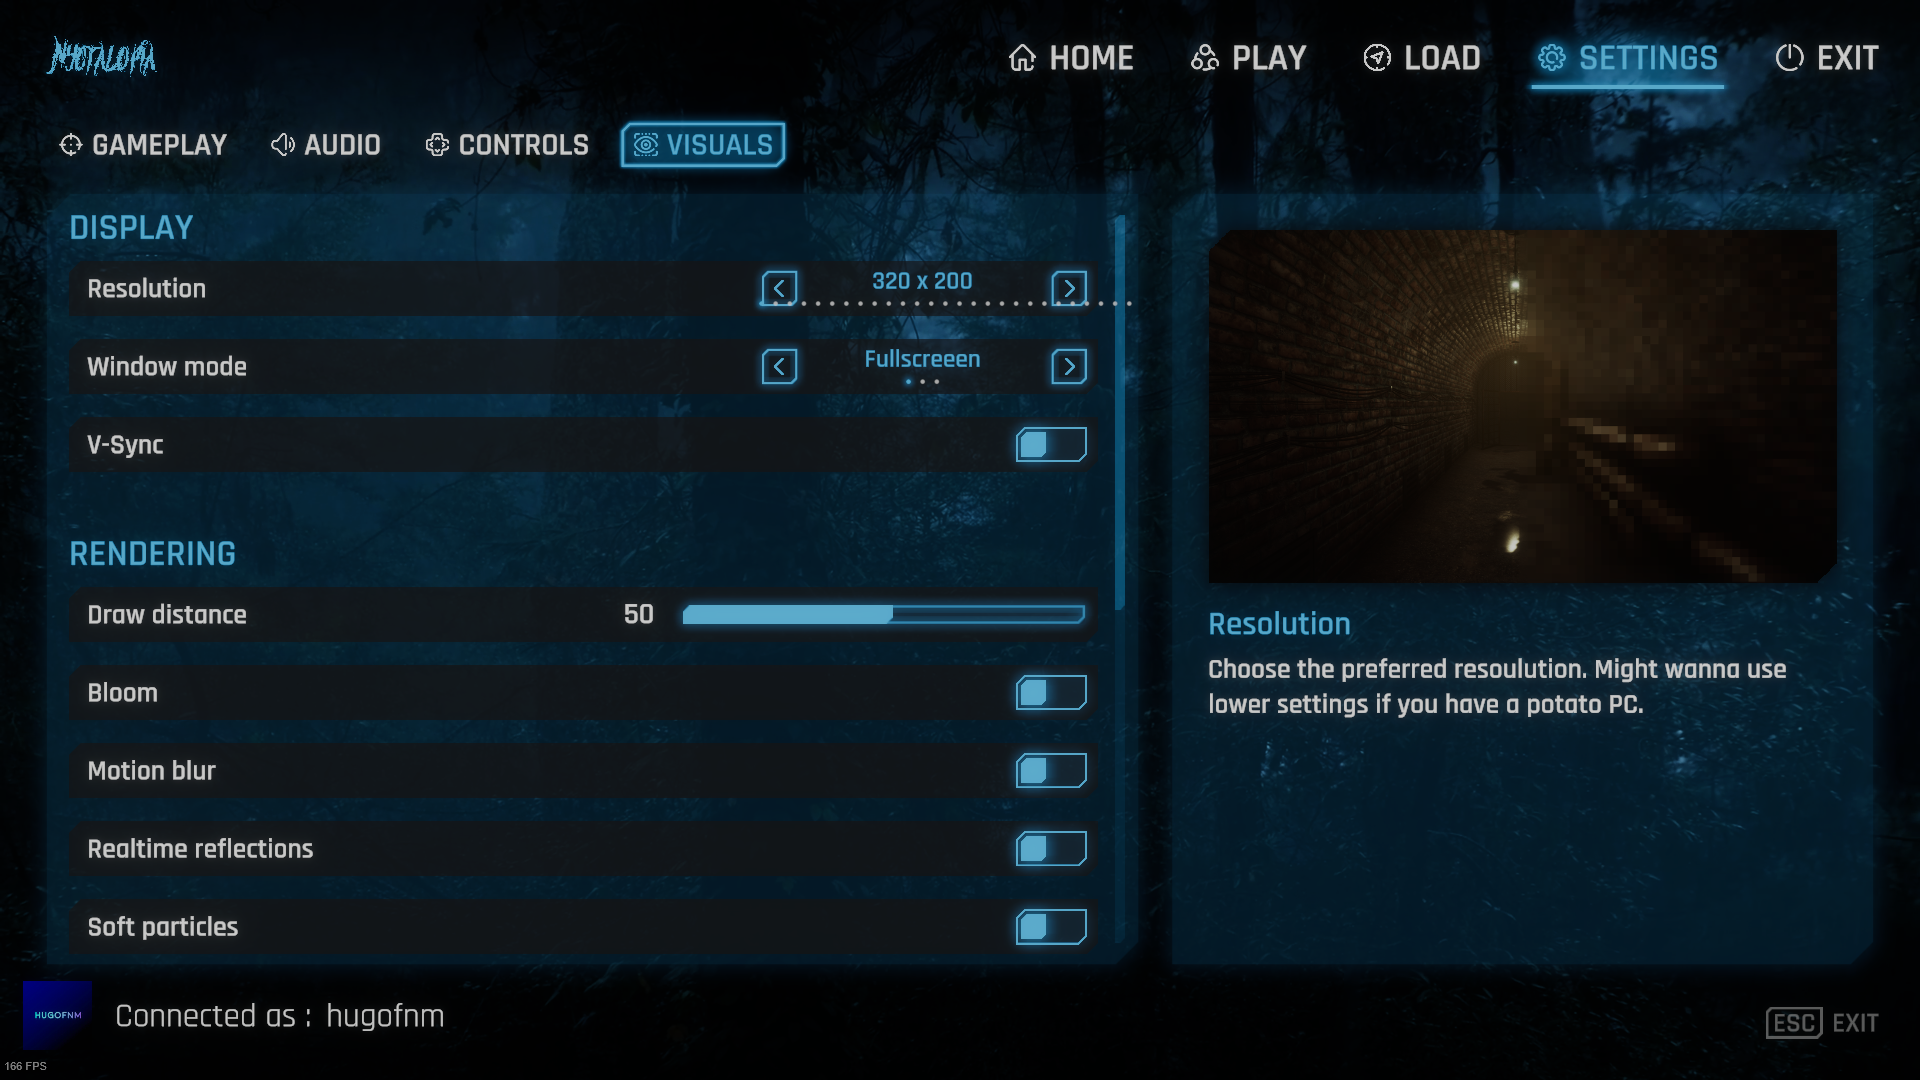
\includegraphics[width=.9\linewidth]{img/ui/UI4.png}
  \captionof{figure}{\emph{Menu ``Paramètres''}}
  \label{fig:uisettings}
\end{minipage}
\end{figure}

Nous avons également mis en place un installateur graphique \emph{``.exe''} qui est accessible à tout utilisateur possédant une machine Windows 10 ou 11 64 Bits sur le site \emph{nyctalopia.games} ou bien grâce à un lien direct avec une redirection HTTP 301 vers des artifacts CI/CD : \emph{get.nyctalopia.games}.
Nous comptons également à mettre en place une version Linux, comme le stipule le sujet, qui sera disponible sur \emph{linux.get.nyctalopia.games} qui renvoie aussi sur un téléchargement direct depuis le CI/CD GitLab Nyctalopia \emph{gitlab.nyctalopia.games} (c.f Site Web).

\begin{figure}[H]
\centering
\begin{minipage}{.5\textwidth}
  \centering
  \centerline{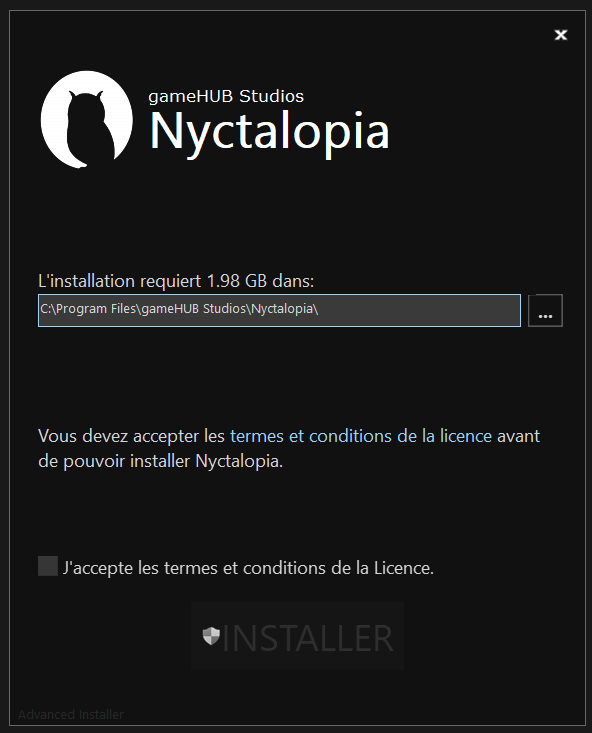
\includegraphics[width=1.5\linewidth]{img/ui/installer.png}}
  \captionof{figure}{\emph{Installateur Graphique \emph{.exe}}}
  \label{fig:uiinstaller}
\end{minipage}%
\end{figure}

\subsection{Site Web}
\setlength{\parindent}{5ex}
Lorem ipsum dolor sit amet, consectetur adipiscing elit. Integer fermentum eros sed neque aliquet fermentum. Ut aliquam placerat velit. Vestibulum ante ipsum primis in faucibus orci luctus et ultrices posuere cubilia curae; Etiam interdum in erat vitae convallis. Nullam sed mauris in ex porta auctor. Aenean in lobortis mi. Nam molestie felis sit amet maximus congue. Aenean rhoncus, libero nec suscipit aliquam, risus velit ultricies est, at vestibulum ipsum elit sed risus. In malesuada efficitur ipsum vel vestibulum. Integer sed mi nec augue laoreet efficitur vel et risus. Quisque pharetra nunc elit.

% NE PAS TOUCHER A PARTIR DICI MARIN STP :)

\begin{figure}[H]
\centering
\begin{minipage}{.5\textwidth}
  \centering
  \centerline{
\includegraphics[width=1.5\linewidth]{img/ssl.png}}
  \captionof{figure}{\emph{Site sécurisé SSL}}
  \label{fig:dns}
\end{minipage}%
\end{figure}

Le site web est hébergé sur CloudFlare Pages, un service gratuit de l'entreprise de gestion DNS CloudFlare, permettant de déployer rapidement à partir d'un repo Git, un site web statique rapide grâce aux serveurs CDN disposés partout dans le monde et sécurisé par un certificat SSL et une protection anti-DDOS.
Le nom de domaine choisi est \emph{nyctalopia.games}. Il est simple et facile à retenir pour l'utilisateur.

\begin{figure}[H]
\centering
\begin{minipage}{.5\textwidth}
  \centering
  \centerline{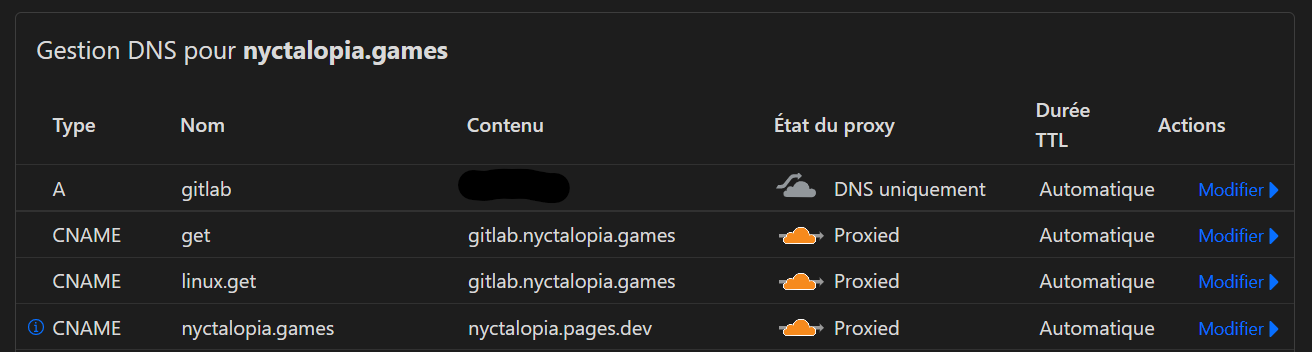
\includegraphics[width=2\linewidth]{img/ui/dns.png}}
  \captionof{figure}{\emph{Interface CloudFlare}}
  \label{fig:dns}
\end{minipage}%
\end{figure}

Nous avons également décidé de mettre en place un GitLab (\emph{gitlab.nyctalopia.games}) privé sur un serveur nous appartenant, ce qui nous a permis d'utiliser la puissance brute de Git LFS et des pipelines CI/CD, améliorant notre productivité sans perdre de temps.

\vfill
\noindent\makebox[\linewidth]{\rule{.8\paperwidth}{.6pt}}\\[0.2cm]
EPITA Toulouse - Projet S2 - 2022 \hfill Nyctalopia - gameHUB
\noindent\makebox[\linewidth]{\rule{.8\paperwidth}{.6pt}}

\newpage